\newcommand{\versionnumber}{0.2}
\newcommand{\docversion}{
  \renewcommand{\arraystretch}{0.5}
  \setlength{\tabcolsep}{0pt}
  \begin{tabular}[b]{l}
  Versie \versionnumber{}\\
  \today \\
  \end{tabular}
}
\newcommand{\doctitle}{KBS ESA3 \\ Eindverslag \\ Smart Markers}
\newcommand{\doctitleshort}{Eindverslag - Smart Markers}
\newcommand{\docauthor}{
  \renewcommand{\arraystretch}{0.5}
  \begin{tabular}{l l}
  Jerko Lenstra & {\mdseries(S1080179)} \\
  Rick de Bondt & {\mdseries(S1078239)} \\
  Marthijn Tijmes & {\mdseries(S1063534)} \\
  \end{tabular}
}

\newcommand{\doctitlepage}{
  \thispagestyle{empty}

  \parbox[t]{1.0\linewidth}{
    \fontsize{40pt}{60pt}\selectfont
    \doctitle{}
    \fontsize{20pt}{40pt}\selectfont
    \\hbo-ICT, Windesheim
    \\Docent: Gido Hakvoort
  }

  \setlength{\wpYoffset}{-1.8cm}
  \ThisCenterWallPaper{0.75}{final_report/windesheim_kadaster.png}
  \vfill

  {
   \docversion{}
   \hspace{185pt}
   \docauthor{}
  }

  \normalcolor{}

  \newpage
}

\providecommand{\doctitle}{Title}
\providecommand{\docauthor}{Author}
\providecommand{\doctype}{scrartcl}
\providecommand{\doctitlepage}{TitlePage}

\documentclass[12pt,a4paper,titlepage,parskip=half]{\doctype}

\usepackage[dutch]{babel}
\usepackage{blindtext}
\usepackage{float}
\usepackage[hidelinks]{hyperref}
\usepackage{graphicx}
\usepackage{listings}
\usepackage{wallpaper}
\usepackage[headsepline,footsepline,manualmark]{scrlayer-scrpage}


% Input and output encoding ---------------------------------------------------
\usepackage{iftex}
\ifPDFTeX
   \usepackage[utf8]{inputenc}
   \usepackage[T1]{fontenc}
   \usepackage{lmodern}
\else
   \ifXeTeX
     \usepackage{xltxtra}
   \else
     \usepackage{luatextra}
   \fi
   \defaultfontfeatures{Ligatures=TeX}
\fi

% Math
\usepackage{amsmath}
\usepackage{amsfonts}
\usepackage{amsthm}
\usepackage{amssymb}
\usepackage{mathtools}

\DeclarePairedDelimiter{\ceil}{\lceil}{\rceil}
\DeclarePairedDelimiter{\floor}{\lfloor}{\rfloor}
\DeclarePairedDelimiter{\bag}{\langle}{\rangle}
\DeclarePairedDelimiter{\set}{\{}{\}}

% Misc
\usepackage[shortlabels]{enumitem}
\usepackage{pgfgantt}

% Bibliography
\usepackage{csquotes}
\usepackage[natbib,style=apa,citestyle=authoryear]{biblatex}
\DeclareLanguageMapping{dutch}{dutch-apa}
\defbibheading{bibliography}[\bibname]{\section{#1}}
\addbibresource{final_report/bibliography.bib}

% Display
\usepackage{lastpage}
\usepackage{tabularx}
\setlength{\headheight}{24pt}

\title{\doctitle}
\author{\docauthor}
\date{\today}

\ihead{\upshape{\doctitleshort}}
\ohead{\upshape{\today, v\versionnumber}}
\cfoot{\upshape{\thepage\ /~\pageref{LastPage}}}

\numberwithin{equation}{section}
\numberwithin{figure}{section}
\numberwithin{table}{section}

\usepackage{changepage}

\usepackage{enumitem}
\setitemize{noitemsep,topsep=0pt,parsep=0pt,partopsep=0pt}

% UML
\usepackage[T1]{fontenc}
\usepackage[utf8]{inputenc}
\usepackage{fancyvrb}
\usetikzlibrary{positioning}
\usepackage{tikz-uml}

%Other settings
\lstset{basicstyle=\ttfamily}

\RedeclareSectionCommand[beforeskip=1\baselineskip,
                         afterskip=.25\baselineskip]{section}

\RedeclareSectionCommand[beforeskip=.25\baselineskip,
                         afterskip=.25\baselineskip]{subsection}

\RedeclareSectionCommand[beforeskip=.25\baselineskip,
                         afterskip=.25\baselineskip]{subsubsection}

\RedeclareSectionCommand[beforeskip=.25\baselineskip,
                         afterskip=.25\baselineskip]{paragraph}

\begin{document}
\doctitlepage{}

\tableofcontents
\thispagestyle{empty}
\newpage

\clearpage
\setcounter{page}{1}
\addtocontents{toc}{\protect\thispagestyle{empty}}

\newpage
\section{Documenthistorie}

\begin{tabularx}{\textwidth}{| l | l | X | l |}
    \hline
    \textbf{Versie} & \textbf{Datum} & \textbf{Verandering} & \textbf{Auteur(s)}
    \\ \hline
    0.1	& 11-jan-2018 & Aanmaken document & Jerko Lenstra \\ \hline
    0.2 & 12-jan-2018 & Toevoegen Product, Proces, Ethische aspecten en Security
     & Marthijn Tijmes \\ \hline

\end{tabularx}


\newpage
\section{Inleiding}
In Nederland is het vanzelfsprekend dat vastgoed geregistreerd is en dat er bekend
is welke gegevens bij dat vastgoed horen. Het Kadaster is verantwoordelijk voor de
vastlegging en verstrekking van vastgoed- en geografische informatie en de rechten
die daarbij horen, zoals eigendom en hypotheek. \citep{KAD_OVER}

Nederland is op gebied van kadastrale registratie vooruitstrevend; in het buitenland
is het niet vanzelfsprekend dat gegevens van vastgoed ergens zijn vastgelegd.
Als gevolg daarvan kan men in deze landen niet aantonen wat hun ontroerend goed is
of wat de waarde daarvan is.

Uit de morele overtuiging dat iedereen recht op eigendom heeft, wat onder andere
opgenomen is in artikel 17 van de Universele Verklaring van de Rechten van
de Mens (UVRM) \citep{UN_UDHR}, wil het Kadaster International deze landen een systeem bieden waarmee
deze eigendommen in kaart gebracht kunnen worden. Dit systeem is recentelijk in
ontwikkeling genomen en het project draagt de naam: \textit{Smart Markers}

\subsection{Aanleiding}
Door het Internet-of-Things keuzesemester van de opleiding hbo-ICT, te Windesheim,
zijn de uitvoerende studenten in aanraking gekomen met dit project. Tijdens het
keuzesemester is er een periode van tien weken waarin studenten aan een project
werken wat in het kader staat van (inter)connectiviteit, duurzaamheid en in het
belang is van de maatschappij.

\subsection{Doel}
Het doel van het project is om ontwikkelingslanden een systeem te bieden dat
een soortgelijke werking heeft als de kadastrale registratie van het Kadaster
in Nederland.

Binnen de scope van tien weken betekent dit het ontwikkelen van een prototype
van een systeem waar locatiegegevens mee kunnen worden verzameld. In hoofdstuk
\ref{sec:opdracht} wordt dit systeem verder uitgediept.


\newpage
\section{Product}
\subsection{Ontwerp}
Tijdens de ontwerpfase is er gesproken over een mesh netwerk van GPS-modules, die
communiceren via LoRa, echter is er relatief vlot besloten om een simpelere
implementatie uit te werken, in verband met de korte tijdsduur van het project.

Het bijgestelde doel was om een prototype van een systeem te ontwikkelen dat
locatiegegevens kan meten, registreren in een database en een simpele dataweergave
te tonen.

\subsection{Status}
Momenteel kan het prototype de locatie uit de GPS halen middels I2C communicatie
en deze middels SPI doorgeven aan de LoRa module. De onderstaande foto weergeeft
een testmeting, die op 1-2m nauwkeurig is.

\begin{center}
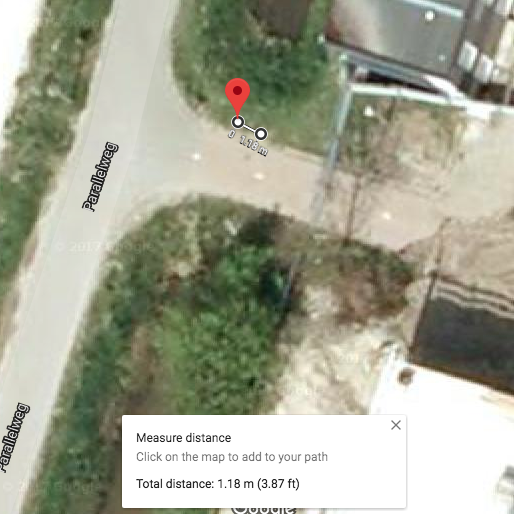
\includegraphics[width=0.5\linewidth]{final_report/measurement0.png}
\end{center}

Via de KPN Portal komt het binnen bij onze API, waar de binnengekomen berichten
in de database gelogd worden. Vanaf de KPN naar onze server loopt het verkeer via
een HTTPS verbinding.

De server draait op CentOS7, waarbinnen een Apache webserver en een MariaDB SQL-
server draaien om de gegevens op te slaan en te verwerken.

\newpage
Verder is de server in staat om van de meetpunten een kaart te tonen op een
webpagina. Hierop zijn de meetpunten te selecteren om toe te voegen aan een perceel.

\begin{center}
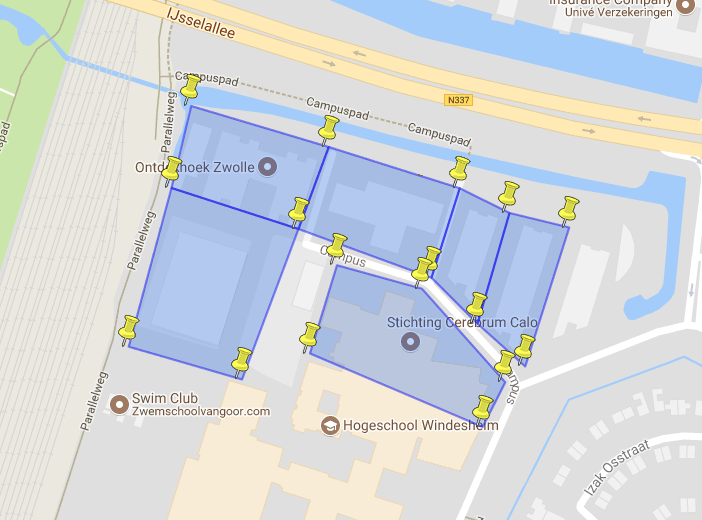
\includegraphics[width=0.5\linewidth]{final_report/webpage.png}
\end{center}

\subsection{Advies}
In deze ontwikkelfase wordt er nog gebruik gemaakt van het KPN LoRa netwerk, wat
natuurlijk in de doelgebieden niet beschikbaar is. Daarom zal er daar met een
eigen gateway en lokale server gewerkt moeten worden om de GPS-data van de Smart
Markers te verzamelen en verwerken.

Daarnaast kan de energievoorziening gerealiseerd worden, op dit moment is het
prototype alleen in gebruik geweest met een laptop. Te denken valt aan een
(interne), oplaadbare, stroomvoorziening om de marker makkelijker in het veld te
kunnen plaatsen.

Verder hebben we het met het Kadaster gehad over manieren om de percelen met
minder handwerk te maken, bijvoorbeeld door het analyseren van sattelietbeelden.

\subsection{Systeemoverzicht}
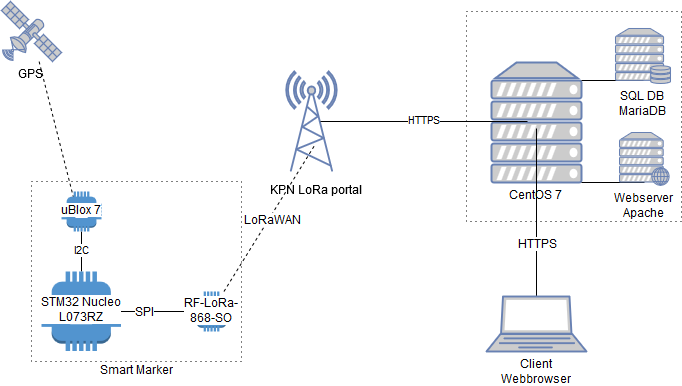
\includegraphics[width=\linewidth]{final_report/system_architecture.png}


\newpage
\section{Proces}
Aan het begin was besloten om het project grofweg in drie delen te knippen:

\subsection{Takenverdeling}
Jerko zou zich vooral richten op de LoRa communicatie en het verzenden van data

Rick zou zich vooral richten op het communiceren met de GPS-module en hier
betrouwbare metingen uit krijgen

Marthijn zou zich vooral bezig houden met het ontvangen en verwerken van de
verzonden data en het combineren van de hardware

Achteraf bleken met name het versturen van data en het communiceren met de
GPS-modules veel meer tijd te kosten dan verwacht, met vele problemen daarbij.
Door de verdeling zijn er grote verschillen ontstaan in kennis van de
verschillende onderdelen, waardoor elkaar helpen af en toe ook erg lastig was.
Het was beter geweest om het in kleinere blokken op te delen en elkaar meer te
betrekken bij de verschillende onderdelen en daarbij behorende problemen.


\newpage
\section{Ethische aspecten}
\subsection{Duurzaamheid}
Wat betreft de duurzaamheid hebben we gekozen voor een STM variant welke in een
heel zuinige sleepmode gezet kan worden. Op deze manier zal er zo min mogelijk
energie verbruikt gaan worden door de Smart Markers.

Voor de energievoorziening werd er aan oplaadbare 18650 cellen gedacht. De
markers komen met grote regelmaat weer terug uit het veld, waardoor het erg
simpel is deze cellen tussentijds op te laden. Dit kan uiteraard met groene
energie.

Het idee is dat de markers los van hun voet gehaald kunnen worden, zodat deze,
indien gewenst, achter kan blijven als markering. De marker zelf is meerdere
keren te gebruiken en zal dus vele metingen uit kunnen voeren. Daardoor hoeven
er relatief weinig gemaakt te worden.

\subsection{Welzijn}
In de Universele Verklaring van de Rechten van de Mens (UVRM) van de Verenigde
Naties staat dat iedereen recht heeft op eigendom. Het eigendom van de grond, en
dat op papier bevestigd hebben, draagt daar natuurlijk enorm aan bij.
Bij geschillen en conflicten kan het enorm helpen om duidelijk te hebben waar
grenzen lopen en wie welk perceel in eigendom heeft. Dit is nu vaak al wel
lokaal bekend maar het centraliseren van deze informatie zal naar verwachting
zeker een positieve invloed hebben.

Uiteraard is het natuurlijk niet uit te sluiten dat er conflicten ontstaan door
het in kaart brengen van grenzen, maar omdat de grenzen al bestaan werd verwacht
dat dit geen grote problemen zou opleveren.

\subsection{Gezondheid}
Wat betreft de gezondheid zal de Smart Marker weinig tot geen invloed hebben.
Natuurlijk komen er op een relatief klein gebied kortdurig vele markers te
staan, maar het idee is dat deze, samen met de gateway, na enkele dagen weer
verplaatst worden naar een volgend gebied. De elektromagnetische straling zal,
voor zo ver dit überhaupt invloed heeft, daarom nihil zijn gezien de
tijdsperiode dat de mensen in het gebied hieraan blootgesteld worden.


\newpage
\section{Security}
\textbf{Het verplaatsen van de marker voordat deze zijn locatie doorgestuurd
heeft} \newline
Paul Saers van het Kadaster gaf aan dat dit geen probleem was; hij gaat er
vanuit dat de markers niet verplaatst worden. Hij verwacht dat de goodwill van
de lokale bevolking groot genoeg is om de metingen niet te saboteren.

Eventueel is hier wel op te controleren met een bewegingssensor, waardoor
meetpunten niet verzonden worden of bijvoorbeeld een kenmerk krijgen dat deze
mogelijk onbetrouwbaar zijn.

\textbf{Het onderscheppen van verzonden gegevens} \newline
Gezien de Smart Markers naar alle waarschijnlijkheid op een eigen gateway gaan
werken en het KPN netwerk momenteel alleen gebruikt wordt om te testen, is hier
nog niet veel aandacht aan besteed.

Wel wordt het verkeer versleuteld naar de portal van KPN gestuurd en via een
HTTPS verbinding naar de server, wat de veiligheid al een heel stuk waarborgd.
De server is voorzien van certificaten, op dit moment van Let's Encrypt.org

\textbf{Het inzien van de opgeslagen data} \newline
Op dit moment draait de database op een vrij te benaderen webserver bij één van
de projectleden thuis. De Smart Markers zullen naar alle waarschijnlijkheid een
lokale server bij de gateway hebben om de data op te slaan, welke dan niet vanaf
het internet te benaderen is.

Wel is het natuurlijk mogelijk om de website af te schermen met een inlog, zodat
het niet mogelijk is om zomaar de data in te zien. Voor het gemak van het
project en gezien het feit dat we nu nog geen gevoelige data verwerken hebben we
hier nog niet voor gekozen.

Daarnaast is de veiligheid van de database te vergroten door enkel vanaf
localhost (de server zelf), eventueel aangevuld met een whitelist van eigen
IP-adressen, inloggen toe te staan. Op dit moment is echter inloggen vanaf elke
locatie mogelijk, gezien de vele plaatsen vanaf waar er gewerkt wordt aan dit
project. In een productieomgeving is dit zwaar af te raden!

\textbf{Het verlies van opgeslagen data} \newline
Peter Brouwer van het Kadaster gaf aan dat eigenlijk overal een (goede)
internetverbinding beschikbaar kan zijn. Het idee was om de lokaal verzamelde
data, wanneer het eenmaal compleet is, te versturen naar een externe bron.
Daarnaast kan het natuurlijk ook lokaal dubbel opgeslagen worden of gebackupt
worden.

\textbf{Onnauwkeurigheid van de meting} \newline
De GPS-ontvangers zelf hebben een indicatie van hoe nauwkeurig ze zijn. Er kan
dus worden besloten om nog niet uit te zenden wanneer deze een (grote) afwijking
heeft. Daarnaast verwachten we dat een langer geplaatste marker, met meerdere
uitgevoerde metingen, ook een betrouwbaarder gemiddelde zal geven.


\newpage
\section{Reflectie}

\subsection{Jerko Lenstra}
Het Smart Markers project vond ik leuk en uitdagend om aan te werken, maar het
project was van veel te korte duur om een goed product neer te kunnen zetten.
We hebben behoorlijk wat moeten schrappen van de projectplanning, omdat er gewoon
geen tijd voor was om het te implementeren. Het leek mij erg leuk om aan de gang
te gaan met een LoRa mesh netwerk te onderzoeken en op te bouwen.

Omdat ik eerder met LoRa heb gewerkt verwachtte ik dat het implementeren van LoRa
erg simpel zou zijn en niet veel tijd in beslag zou nemen, daarom leek het mij
handig voor de gebruiker (Kadaster) om een abstractie laag tussen de LoRaWAN stack
en de gebruiker applicatie te hebben. Dit heeft veel langer geduurd dan verwacht,
en heeft ervoor gezorgd dat op sommige momenten mijn teamgenoten op mij moesten
wachten voordat zij verder konden.

Het KBS is niet altijd even soepel verlopen, omdat geen van ons echte leiderschap
karakteristieken heeft, daardoor was het een uitdaging om op de juiste koers te
blijven, maar volgens mij is het redelijk gelukt. Los van een bug met de timers
die we niet hebben kunnen vinden, hebben we ons doel bereikt en heb ik een hoop
geleerd.

Het was interessant om voor een echt bedrijf een opdracht te mogen doen, maar het
bracht mij ook enige stress mee, omdat de communicatie tussen de opdrachtgever en
ons niet altijd heel helder is geweest. We zijn aan het begin van het project best
veel tijd verloren in het afstemmen van wat de opdracht precies is. Achteraf denk
ik dat het minder chaotisch was geweest als we onze eigen opdracht hadden verzonnen.

\subsection{Rick de Bondt}


\subsection{Marthijn Tijmes}


\newpage
\printbibliography

\end{document}
